% vim: set tw=78 tabstop=4 shiftwidth=4 aw ai:

\chapter{Peer-to-Peer Systems and Protocols}
\label{chapter:p2p-systems}

Peer-to-Peer (P2P) Systems have become a ``buzzword'' in the early 21st
century and are nowadays one of the most common technologies used in the
Internet. Although until 2000 the most common paradigm in Internet was
client-server, the emergence of Napster has pushed Peer-to-Peer systems
to become one of the most used (and controversial) technologies.

With a total of 60 million users in 2001 and many terabytes of music shared,
Napster became the center of public attention and the promoter of P2P
technology. Soon after that a series of Peer-to-Peer solutions led to new
ways of sharing information, files, knowledge and data (JXTA, Gnutella,
BitTorrent, DirectConnect, Jabber).

In its original meaning, ``Peer-to-Peer'' refers to communication between
equals, between two autonomous entities that are independent of each other.
Generally, a ``Peer-to-Peer'' system is a decentralized system: each node in
the network possesses the same role as any other node. The opposite is a
client-server system, which is centralized on the server. An immediate
advantage of Peer-to-Peer architecture is scalability and fault tolerance.

\begin{figure}
  \centering
  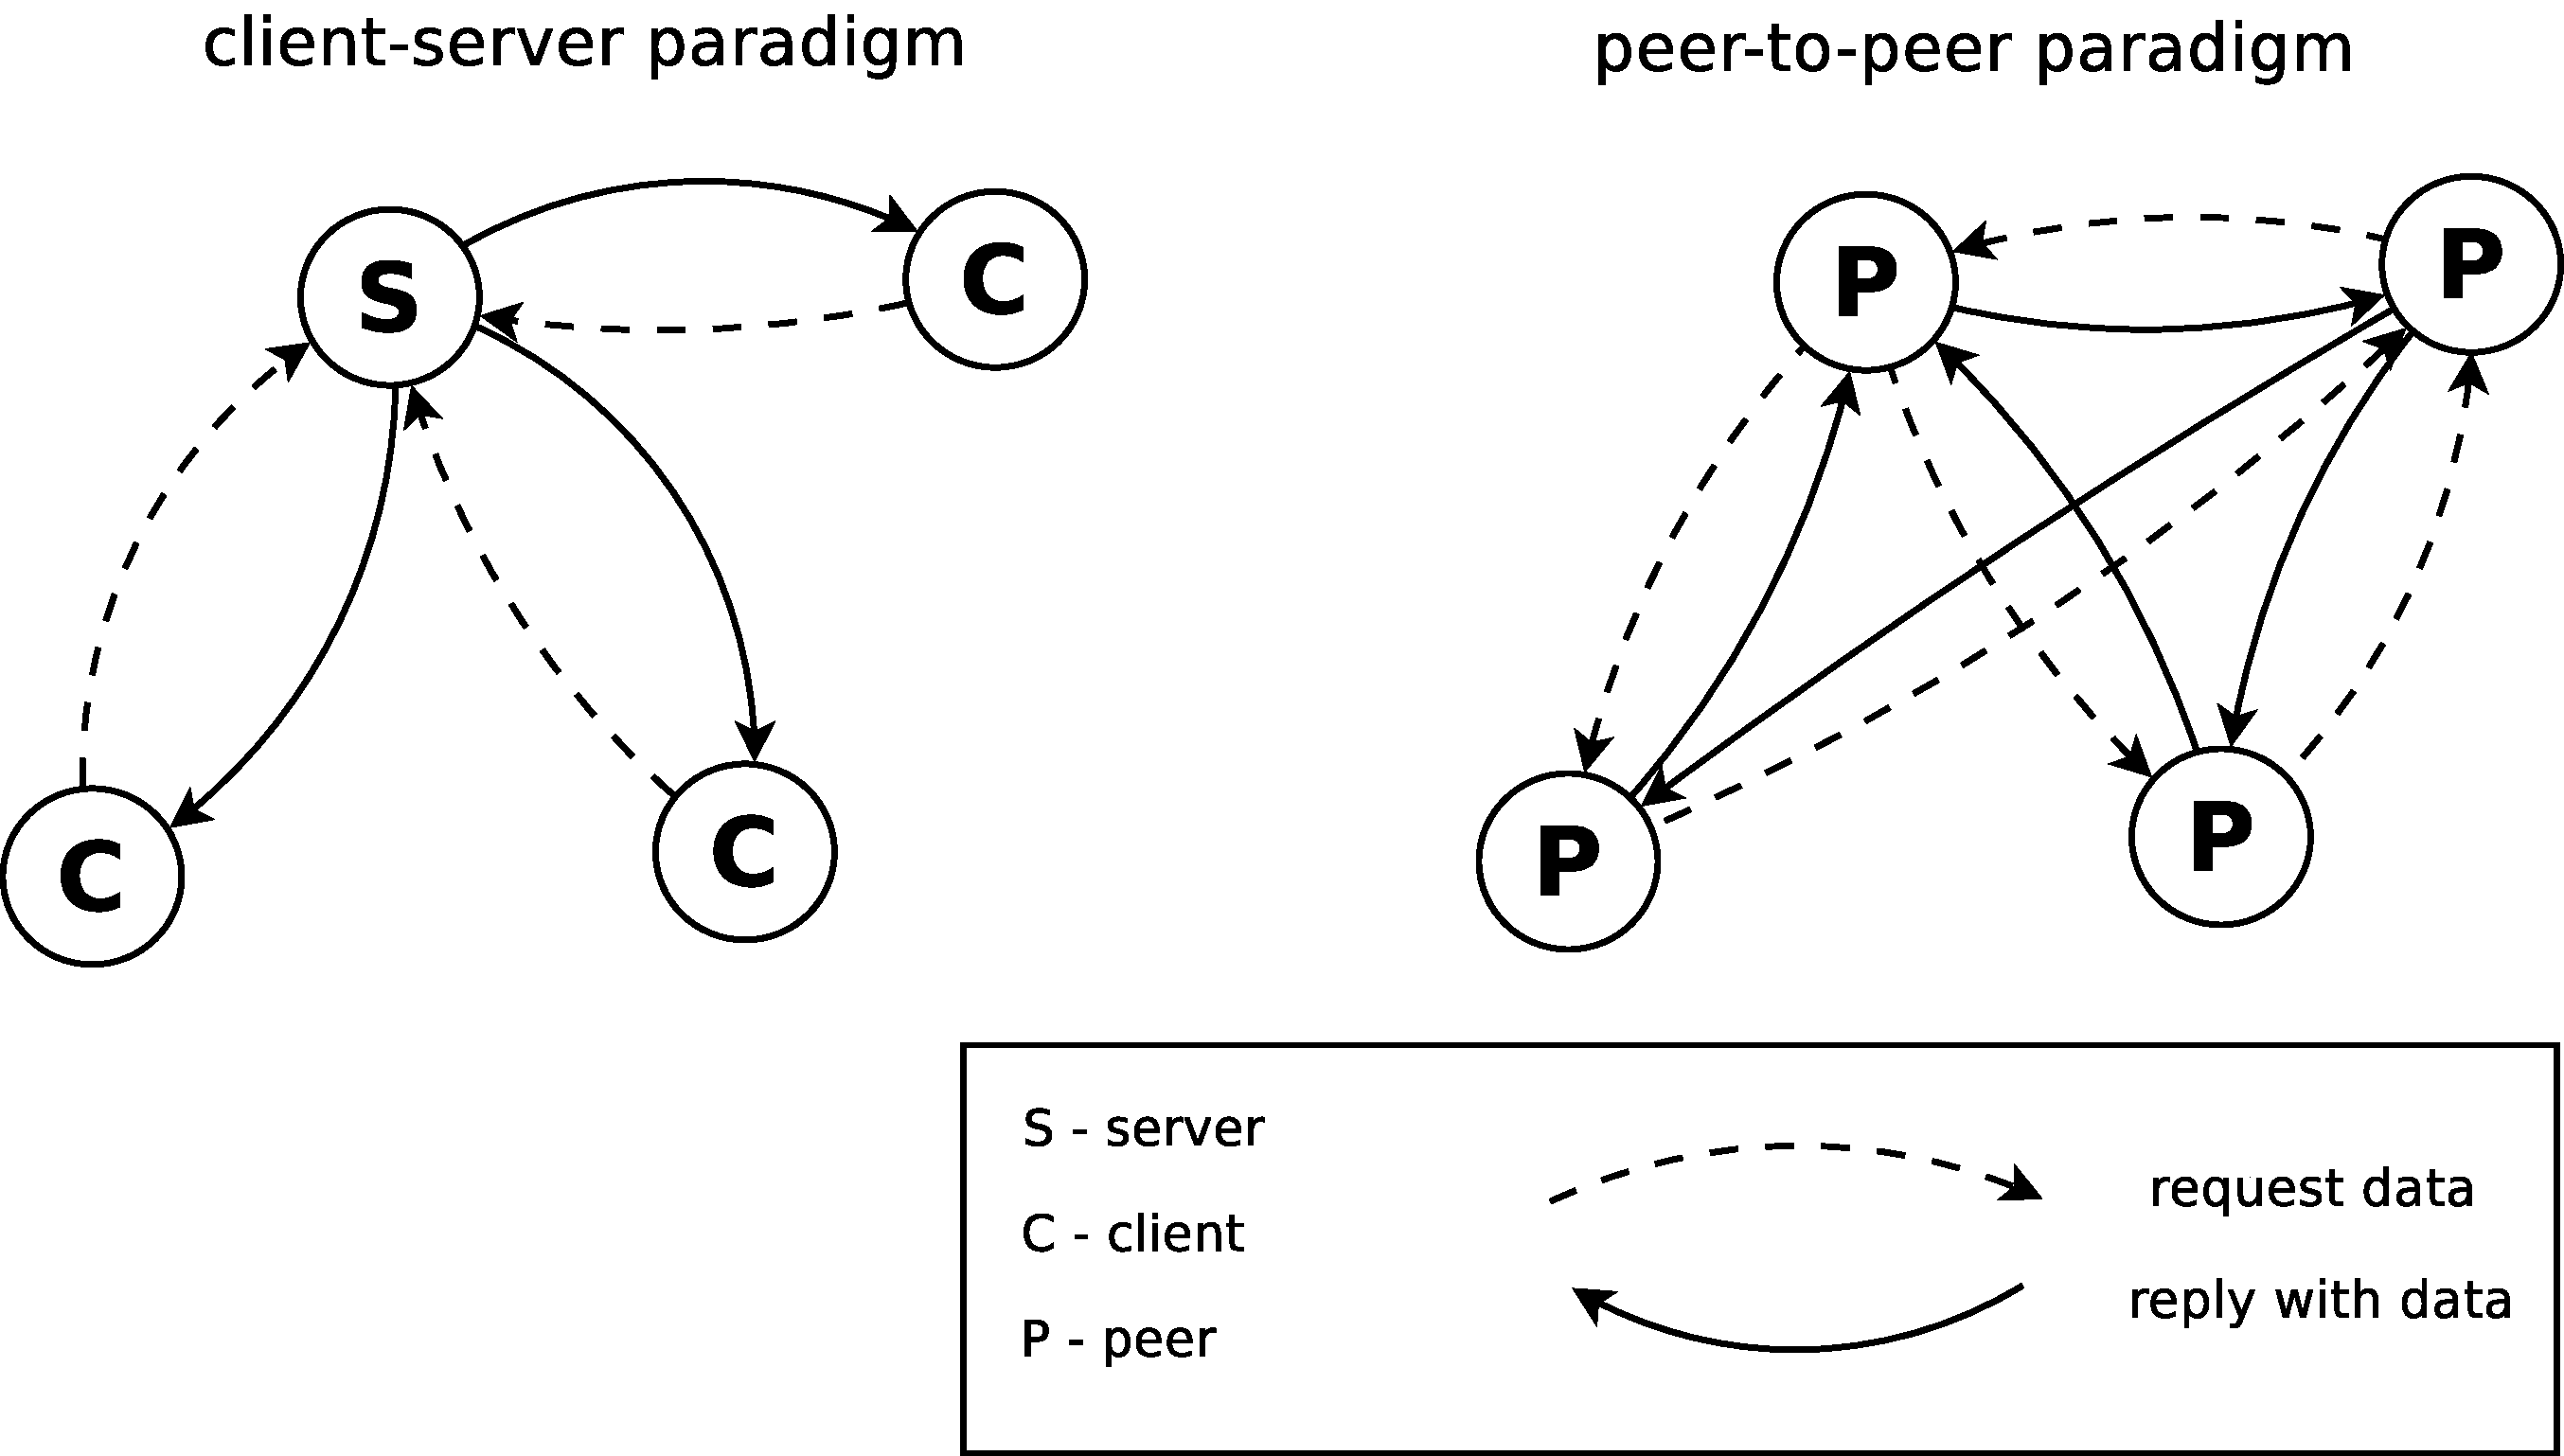
\includegraphics[width=0.7\textwidth]{src/img/p2p-systems/client-server-vs-p2p}
  \caption{Client-Server versus Peer-to-Peer}
  \label{fig:p2p-systems:client-server-vs-p2p}
\end{figure}

In order to claim a system as being ``Peer-to-Peer'', it must provide a
positive response to the following questions:
\begin{itemize}
  \item Does the system deal with variable connectivity and temporary
  addresses as a matter of course?
  \item Does the system provide autonomous visibility for nodes at the edge of
  network?
\end{itemize}

In addition, there is a third default condition, which states that
communication between nodes must exists for the system to work.

It is noticeable that these conditions don't require a decentralized
architecture as Peer-to-Peer systems are usually charged. These conditions
require that each network node is an independent player and its presence
is not mandatory for the system to work.

The Internet is a shared resource, a reservoir of information and a
cooperative network built with millions of nodes worldwide. As of the 90s, the
Internet has experienced an explosive growth which generated an acute demand
for one of the basic network resources: bandwidth. The firewall arose from the
need of supporting a variety of applications with constraints regarding
security.

However, in 2000 everything changed, or, better said, returned to the initial
state. Passive elements have become active elements. Through sharing of music
files (via Napster) and through a larger movement (called Peer-to-Peer),
millions of users connected to the Internet began using their systems
for more than reading e-mails and browsing. Systems connected through the
Internet could form groups and collaborate to meet various needs.

Since 2000 (Napster), Peer-to-Peer applications have become more common and
widely used. Peer-to-Peer applications allow easy publication of information
and designing of decentralized applications, which is simultaneously a
challenge and an opportunity.

In this case, Peer-to-Peer model is closely linked with the idea of
decentralization. In a fully decentralized system, each node is an equal
participant without having any special role. DNS is a Peer-to-Peer protocol
that has the implicit idea of hierarchy. Many other Peer-to-Peer systems have
a semi-centralized organization with some nodes having special roles.

However, Peer-to-Peer applications encounter server problems in the current
Internet architecture: firewalls and NAT make it more difficult to create
connections between stations. Asymmetric bandwidth prevents users from
efficiently serving files from their computers.

Beyond technical problems, Peer-to-Peer applications face social problems.
Sharing files in a Peer-to-Peer system must take into account free-riders.
Free-riders are those who use resources shared by others (files, bandwidth,
memory, CPU power) without giving anything back (or giving to little). The
resulting lack of reciprocity is damaging for the health of the Peer-to-Peer
network. As such, a form of accounting effort for each customer must employed.

At the time, ever since the launch of Napster, Peer-to-Peer applications have
attracted many issues related to sharing copyrighted materials, such as audio,
video, electronic documentation, etc.

\section{The Peer-to-Peer Paradigm}
\label{sec:p2p-systems:paragigm}

The Peer-to-Peer paradigm has established itself as an alternative (if not
opposite) to the client-server paradigm. Providing scalability and taking
advantage of the continuous increase in Internet network bandwidth, the
Peer-to-Peer paradigm has been in various situations such as file sharing,
communication, collaboration, social networking, load distribution.

\subsection{Features and Models of Peer-to-Peer Systems}

As mentioned previously, the characteristics of P2P networks are sharing and
distribution of resources, decentralization and autonomy.

Sharing and distribution of resources refers to the functionality provided by
each node of the Peer-to-Peer network. A node can function as a server or as a
client and may also act as a provider and consumer of resources and
services (information, files, bandwidth, storage, processor cycles). These
nodes are also called ``servants''.

Decentralization refers to the absence of a central coordinating authority for
organizing the network or for resource usage and distribution or communication
between nodes. Communication takes place directly between nodes. There is a
frequent distinction between pure P2P networks and hybrid networks. In
hybrid P2P networks, certain functions (such as indexing and authentication)
are allocated to a subset of nodes that have coordinating role.

Autonomy means that each node independently decides what resources it provides
to other nodes.

The lower cost of CPU power, bandwidth and storage space, combined with
the growth of the Internet have created new areas for applying P2P networks.
This has led to an explosive growth of P2P applications and to discussions about
limitations, performance and economic, social and legal topics.
Figure~\ref{fig:p2p-systems:p2p-levels} shows a model based on P2P
infrastructures, applications and communities.

\begin{figure}
  \centering
  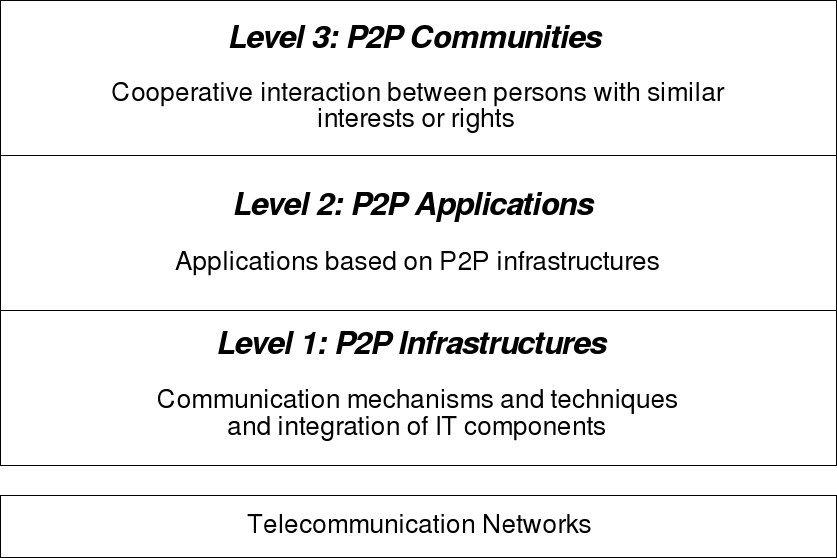
\includegraphics[width=0.7\textwidth]{src/img/p2p-systems/p2p-levels}
  \caption{Peer-to-Peer Levels}
  \label{fig:p2p-systems:p2p-levels}
\end{figure}

P2P infrastructures are positioned over existing communication networks and
acts as a foundation for other levels. P2P infrastructures provide
communication, integration and translation between various IT components. It
also provides search services, communication and sharing between network
nodes and initiation of security processes such as authentication and
authorization.

Level 2 is represented by P2P applications that use P2P infrastructure
services. Applications are used to allow communication and collaboration
among different entities in the absence of a central supervisor/coordinating
node.

Level 3 focuses on the social networking phenomenon; in particular, on
building communities and their dynamics.

\subsection{P2P Resource Management}

In specialized literature, P2P applications are often classified in categories
such as: instant messaging, file sharing, grid computing and collaboration.
This classification has been developed over time and fails to make clear
distinctions between different applications. Nowadays there are many
situations where several categories may be considered equivalent. For these
reasons, another classification could take into account issues regarding
resources usage in P2P systems.

As such, there is a classification of P2P systems regarding available resources.

\subsubsection{Data}

Information is used in collaborative spaces in the form of sharing or
exchanging information and document management. Information about the presence
of nodes in P2P systems is fundamental for the organization of a P2P system
and for knowledge of resources they make available. Information regarding
presence useful to knowledge of free CPU cycles on a computer system that may
be used in a grid application.

DMS (Document Management Systems) are storage spaces that enable shared
storage, management and use of data. Formation of collaborative groups for
document management is a result of information-sharing applications (P2P
groupware). In client-server groupware systems, a workspace for the
information management is needed. A P2P system can avoid all tasks related to
the administration of that workspace.

\subsubsection{Files}

Sharing files is the most common form of P2P applications. 70\% of the
Internet traffic may be attributed to file exchange (mostly media files). One
of the main problems of P2P systems (and file sharing applications) is
localizing resources. In the context of file sharing, P2P systems have been
developed three algorithms: flood model, centralized directory model and
conveyance documents model. These models are best illustrated by prominent
implementations such as Gnutella, Napster and Freenet.

\subsubsection{Bandwidth}

With increasing demand for transmission capacity of networks (mainly due to
increasing multimedia transfer) effective use of bandwidth becomes more
important. Usually, a centralized approach, where files are kept on the
server, leads to the occurrence of a bottleneck in the network; the
bottleneck is generated by a set of requests being sent simultaneously from
multiple clients to a single one.

In these situations, using a P2P systems have two advantages:
\begin{itemize}
  \item increasing load balancing through the use of unexploited transmission
  routes;
  \item usage of shared bandwidth that implies acceleration of download speed
  and rapid transfer of large files simultaneously requested by various
  entities.
\end{itemize}

Commonly, files are divided into small blocks downloaded simultaneously from
different nodes of the network.

\subsubsection{Storage}

Increasing connectivity and bandwidth availability allows alternative forms of
storage management that solves these problems and requires less administrative
effort. In P2P storage networks, only a portion of a desktop PC space will be
used. A P2P storage network is a cluster of computers based on networks sharing
existing storage. When a file is stored in the network, a unique identification
number (obtained by applying a hash function on the content of file name) is
assigned to it. In addition, a number of copies of the file are also stored on
the network.

\subsubsection{CPU Cycles}

Realising that computer networks possess a large quantity of unused computing
power, a decision was made to engage P2P applications in using that power.
Using P2P applications for collecting CPU cycles allows a potential higher use
of computing power; such power may be difficult to be provided even with the
employment of expensive supercomputers. The approach of using coordinated
resources of distributed computing that extend beyond a simple institution
falls under the auspices of the domain ``grid computing''.

One of the most common examples of grid projects in the context of P2P networks
if SETI@home. SETI@home is a scientific initiative launched by University of
California, Berkeley, in order to discover radio signals from extraterrestrial
intelligence. For this purpose, a radio telescope from Puerto Rico records a
portion of the electromagnetic spectrum space. Data is transmitted to the
central server based in California. Instead of analyzing data using
supercomputers, the server divides the information into small units and sends
them for processing to millions of computers volunteering to participate in
this project.

\subsection{P2P Topologies for File Sharing}

Topology of P2P systems refers to:
\begin{itemize}
  \item how nodes are connected;
  \item the existence of specialized nodes;
  \item transfer mode for shared file or meta-information.
\end{itemize}

In terms of network topology, P2P systems have two main characteristics:

\begin{itemize}
  \item \textbf{scalability}: there is no technical or algorithmic limitation
  for the system size; system complexity must be relatively constant compared
  to the number of nodes in the system;
  \item \textbf{reliability}: the absence of a given node or its poor
  performance will not affect the whole system (if possible, neither of the
  other nodes).
\end{itemize}

P2P systems may be grouped into two categories: puee P2P systems and hybrid
P2P. \textbf{Pure P2P systems} (such as Gnutella or Freenet) possess no
central server. \textbf{The hybrid P2P model} (such as Napster, eDonkey2000 or
Groove) uses a central server to obtain meta-information or to verify
credentials. In a hybrid system, nodes always contact a central server before
directly contacting other nodes.

All P2P topologies, regardless of differences, have one common feature: all
data transfer sessions between nodes are achieved through direct connection
between nodes. However, controlling the process may be implemented in several
ways. As a result, P2P networks may be classified into four major categories:
centralized, decentralized, hierarchical and ring. Although these topologies
can exist by themselves (independent), distributed systems use more complex
topologies by combining some basic systems into creating what is usually
referred to as a hybrid system.

\subsubsection{Centralized}

Centralized topology concept is based on the traditional client-server
paradigm. There must be a central server used to manage files and databases
of user nodes that enter the system. Clients contact the server to
inform about their current IP address and the file names wanting to share.
This is performed whenever the application is launched. Information collected
from nodes will subsequently be used by the server to create a centralized
dynamic database that maps file names with sets of IP addresses.

\begin{figure}
  \centering
  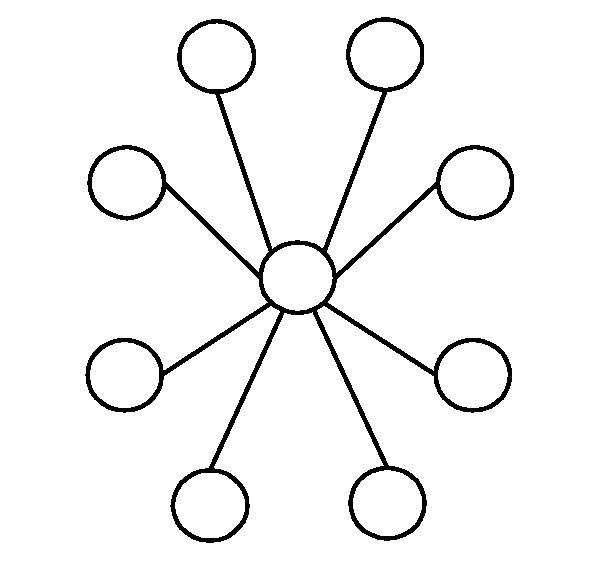
\includegraphics[width=0.4\textwidth]{src/img/p2p-systems/centralized}
  \caption{Centralized Topology}
  \label{fig:p2p-systems:centralized}
\end{figure}

All search requests are submitted to the server which will consult its local
database. If a match occurs, it creates a direct link to the node sharing the
file and run the transfer. In no situation will the shared file be present on
the server.

\subsubsection{Ring}

The most important disadvantage of a centralized topology is the central
server; it can easily become a bottleneck in the system (in case of a heavy
load from client requests) and a critical point in case of failure. As a way
to circumvent the disadvantage, ring topologies have appeared.

\begin{figure}
  \centering
  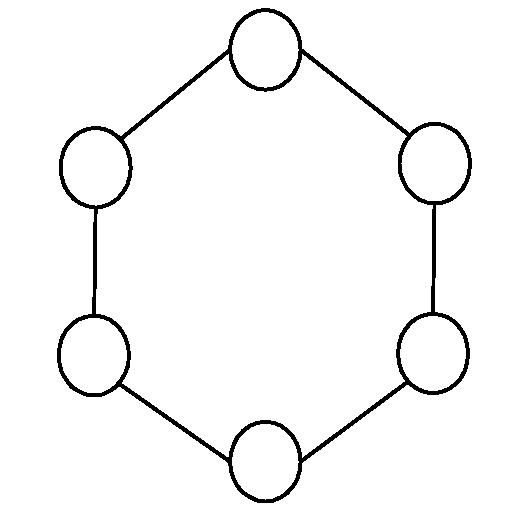
\includegraphics[width=0.4\textwidth]{src/img/p2p-systems/ring}
  \caption{Ring Topology}
  \label{fig:p2p-systems:ring}
\end{figure}

Ring topology is made of a cluster of systems that are arranged in a ring shape
to act as a distributed server. This cluster provides the best possible load
balancing for higher availability. This topology is commonly used when systems
are topologically close and, quite likely, held by a single organization where
anonymity is of little importance.

\subsubsection{Hierarchical}

Hierarchical topologies are probably the most common topological example,
claiming their existence since the beginning of human civilization. The most
famous example of a hierarchical system in the Internet is the DNS
(\texttt{Domain Name System}). Authority delegates from the root name servers
to the registered name server. The topology is suitable for systems that
require a governing entity involving delegation of rights or authority.
Another example is the certification authority (CA) that certifies the
validity of an entry in the Internet, and takes part in the creation of a PKI
(\texttt{Public Key Infrastructure}).

\begin{figure}
  \centering
  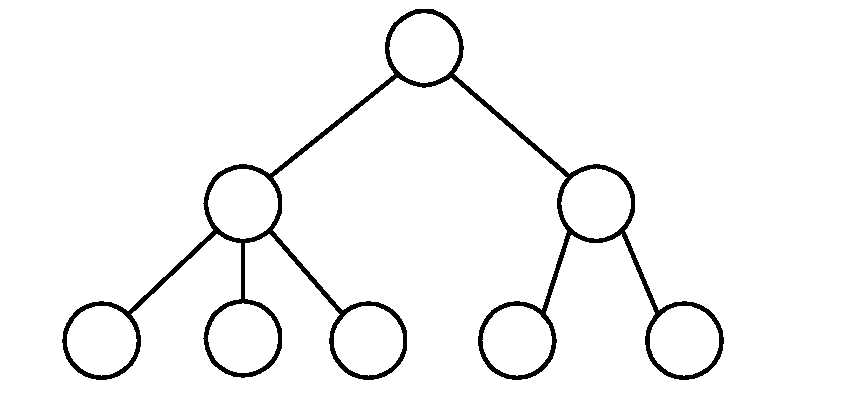
\includegraphics[width=0.4\textwidth]{src/img/p2p-systems/hierarchical}
  \caption{Hierarchical Topology}
  \label{fig:p2p-systems:hierarchical}
\end{figure}

\subsubsection{Fully Decentralized}

In a pure P2P architecture, there are no centralized servers. All nodes are
equal; this ends up in a flat, unstructured topology. In order to join the
network, a node should contact a bootstrap node (a node which is always online).
It will provide to the new node various properties such as IP addresses of one
or more nodes already in the network, making it officially part of the dynamic
network. Most of the time, each node will have only information about its
neighbors -- nodes which are directly connected with it.

\begin{figure}
  \centering
  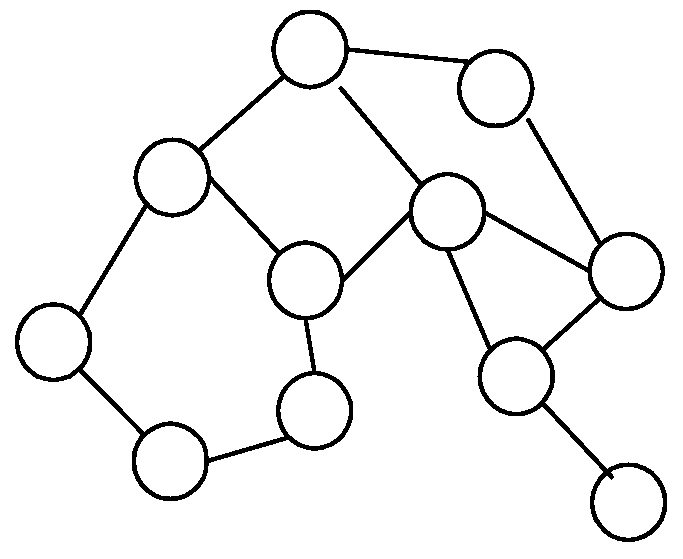
\includegraphics[width=0.4\textwidth]{src/img/p2p-systems/decentralized}
  \caption{Fully Decentralized Topology}
  \label{fig:p2p-systems:decentralized}
\end{figure}

Since there is no control server for searching, file requests are sent in the
form of floods through the network. As a consequence, flooding means additional
load of the network bandwidth.

\subsubsection{Hybrid}

Nowadays P2P networks combine many of the basic topologies shown above; they
are also called hybrid architectures. In such systems, nodes will often play
several roles.

\subsubsection{Centralized Ring}

This hybrid topology is very common for Web hosting systems. As mentioned
previously, Web servers typically have a ring of servers specialized in load
balancing and fault tolerance. As such, web servers providing content for a
single entity/organization are commonly arranged in a ring topology.  Clients
are connected to ring topology using a centralized topology.

\begin{figure}
  \centering
  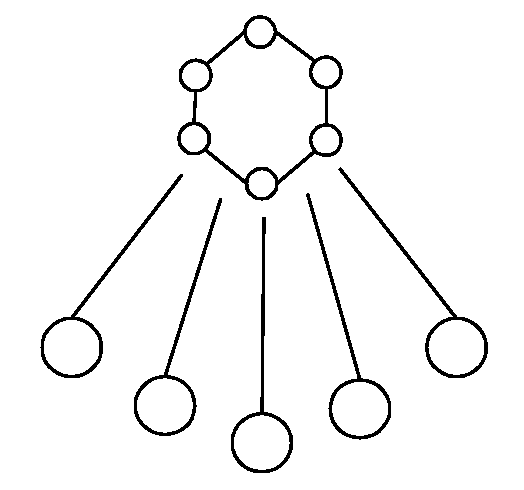
\includegraphics[width=0.4\textwidth]{src/img/p2p-systems/centralized-ring}
  \caption{Centralized Ring Topology}
  \label{fig:p2p-systems:centralized-ring}
\end{figure}

\subsubsection{Centralized-Centralized}

It can often happen that a server of a network is a client in a larger
network. This hybrid topology is also common in organizations that provide
Web services.

\begin{figure}
  \centering
  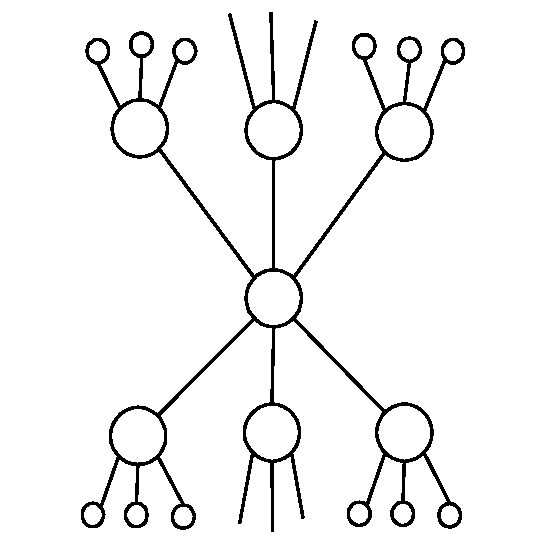
\includegraphics[width=0.4\textwidth]{src/img/p2p-systems/centralized-centralized}
  \caption{Centralized-Centralized Topology}
  \label{fig:p2p-systems:centralized-centralized}
\end{figure}

\subsubsection{Centralized-Decentralized}

In this topology, some nodes function as group leaders (usually called
\textbf{Super-Nodes}). Super-Nodes provide server tasks only in a subset of
nodes  Super-Nodes are connected in a decentralized manner.

\begin{figure}
  \centering
  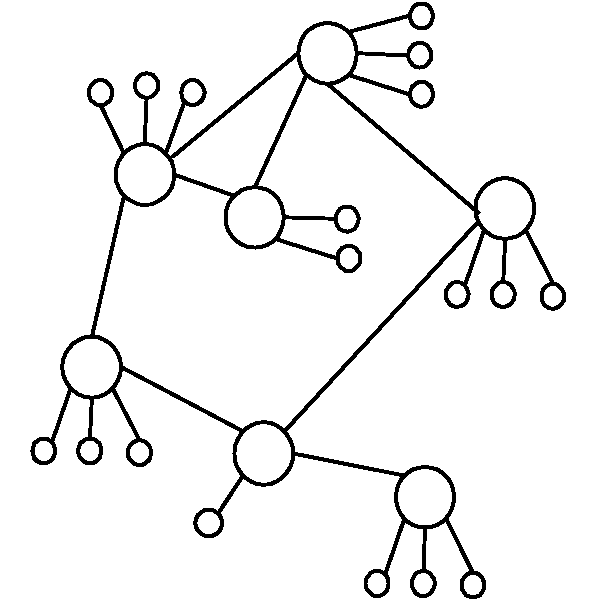
\includegraphics[width=0.4\textwidth]{src/img/p2p-systems/centralized-decentralized}
  \caption{Centralized-Decentralized Topology}
  \label{fig:p2p-systems:centralized-decentralized}
\end{figure}

As in a centralized topology, Super-Nodes maintain a database that maps IP
addresses to files. Super-Nodes database maintains information only about
the group nodes. A sample application that uses such P2P topology is
FastTrack. Another example of such a topology is the e-mail service of the
Internet.

\section{Peer-to-Peer Systems in the Internet}
\label{sec:p2p-systems:p2p-internet}

Starting with Napster's success story in early 2000s, a variety of
Peer-to-Peer solutions have emerged. Though made popular due to the diversity
of P2P file sharing solutions, other applications such as collaborative
software (as in JXTA), video streaming and chat (such as Jabber) have made
their way in the Internet.

Each type of appliation possesses specific features and approach towards
Peer-to-Peer communication. Napster, similar to DirectConnect, provides a
central indexing server, while actual communication (sharing) is enabled
between peers. Gnutella is a fully decentralized approach to file sharing.
Peer connections and interactions require no central server, albeit super
nodes are required to bootstrap the network. BitTorrent, one of the most
successful protocols, isolates a sharing session within a swarm, itself
described by a metadata file, dubbed a \textit{.torrent} file.

\subsection{Napster}

Napster was the first successful example of a Peer-to-Peer system. Napster was
permanently closed in June 2001, an event that marked the end of an
outstanding era, with 65 million users in only 20 months. Napster's central
control model was possible due to focusing user approach.

Figure~\ref{fig:p2p-systems:napster} presents the essential architecture
components of Napster where communication is mediated by the server. Clients
are connecting to a well known \textbf{meta-server}. The meta-server
associates a server with reduced load from one of the clusters. A cluster
consists of 5 servers, each of which can control about 15.000 users.

\begin{figure}
  \centering
  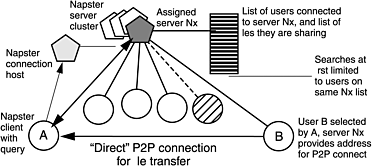
\includegraphics[width=0.7\textwidth]{src/img/p2p-systems/napster}
  \caption{Napster Architecture}
  \label{fig:p2p-systems:napster}
\end{figure}

The client registers to the chosen server, providing information about its
identity and shared files. Afterwards, it receives information about other
online users and available files. Users are anonymous to each other and local
directory structure is not directly interrogated. The main interest is
searching for content and determine where the requested resource may be
downloaded from.  The server directory is only used to translate between
station identity, the desired resource and the IP address necessary to
initiate the connection.

Because network performance is essential, searches are constrained to a maximum
of 100 hits and a maximum of 15 seconds duration. Searches actions take place
in the local database maintained by the server, but, sometimes, may be passed
to neighboring servers within the same cluster.

Conceived originally as a system for sharing MP3 files, a whole culture of
clones and utilities appeared. However, this possesses disadvantages too. For
example, certain tools (such as Wrapster) would be able to make other files
look like MP3 files. Other utilities (such as Napigator) allowed users
connect to certain servers, bypassing the meta-server arbitration phase.

However, even if consistent effort has been put into redesigning Napster, it
still used a centralized and compatible server. This meant a serious
constraint for Napster networks or any other clone implementations. In order
to change this limitation, several protocols and architectures were designed.
These are serverless implementations in the style of Gnutella.

\subsection{Gnutella}

Initially, Gnutella was the name of a prototype client developed in just a few
weeks in March 2000 by the same team that created WinAmp. At its beta version
launching, almost everyone saw Gnutella as a competitor for Napster, designed
to overcome many of its limitations. However, AOL, who had just bought
Nullsoft, decided to immediately stop working on the client. Everything would
have ended if hadn't been Bryan Mayland who managed to deduce Gnutella
protocol and published its specifications on the Internet. Soon began the
development of Gnutella open-source project.

Nowadays Gnutella is a generic term with various meanings: the protocol, the
open-source technology and the Internet network used. There are several
clients for the Gnutella protocol and, although most of them focus on sharing
and searching files, many other operations may be enabled.

Gnutella is mainly a file sharing network that allows arbitrary types of
files. There is no central server and therefore there is no point of failure.
Public or private networks are defined only by clients who are currently in
communication with each other. Each user can build a local map of the network
capturing messages from other clients. There may be multiple networks,
depending on how clients are configured to interconnect.

The lack of a central control point in Gnutella means that legal
responsibility for file transfers remains in user hands. Depending on the
point of view, this may turn out to be a good or a bad thing. On
\textit{gNET}, one may find illegal copies of almost everything one can think
of.

There is no standard client, but there are several clients built on top of the
Gnutella protocol. These clients may communicate with each other, but
developers have liberty for functionalities and extensions implementation.
Gnutella specifications and most of the clients are open-source, but there are
also proprietary implementations.

Authentication in a network like Gnutella is similar to a group of people
looking into different directions. A user only communicates with immediate
neighbors and, through this process, neighbors can communicate with the others.
In each session there is a different selection of people and resources.

Normally a node is able to connect to any node from its neighborhood. But just
like in real life, some nodes may be too busy to talk and will not provide
attention. Other nodes will completely ignore the connection request. Other
nodes will change a few words and will move on. Eventually, it will reach a
node they can establish a long-term contact and to which they can send
requests and results. Nodes appear and disappear continuously and local
configuration requests will change constantly; over time, a node will connect
to multiple nodes.

\begin{figure}
  \centering
  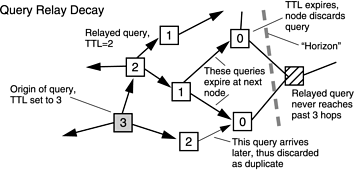
\includegraphics[width=0.7\textwidth]{src/img/p2p-systems/gnutella}
  \caption{Gnutella Architecture}
  \label{fig:p2p-systems:gnutella}
\end{figure}

Atomistic P2P networks such as Gnutella are very dynamic and don't have central
addresses lists. From a pragmatic point of view, a list of bootstrap for initial
discovery is needed.

The inherent virtual network segmentation results in the so called ``horizon
effect''. Each node's visibility is limited to a given number of nodes. In
gNet, this number is 15,000 nodes. Nodes are continuously entering and leaving
the network thus influencing reachable nodes. The main reason for the
occurrence of ``horizon effect'' is the existence of a TTL counter
(\texttt{time-to-live}) similar to IP packets. Typically, TTL is set between 5
and 7 and is decremented by each node through which the message passes. TTL's
value and the number of connected nodes, together with the bandwidth and
capacity of a node, combine to determine the network performance and its
stability. Some clients allow the user to manually adjust the TTL and the
number of active nodes, thus succeeding in expanding the horizon.

Table~\ref{tab:p2p-systems:gnutella-horizon} shows a horizon progress
(number of nodes that can be reached) with respect to TTL value and the number
of nodes connections.

\begin{table}[htb]
  \centering
  \caption{Gnutella Horizon Evolution (number of reachable nodes)}
  \label{tab:p2p-systems:gnutella-horizon}
  \begin{tabular}{@{}lrrrrrr@{}}
    \toprule
      & \textbf{TTL=2} & \textbf{TTL=3} & \textbf{TTL=4} & \textbf{TTL=5} &
      \textbf{TTL=6} & \textbf{TTL=7} \\
    \midrule
      \textbf{N=2} & 4 & 6 & 8 & 10 & 12 & 14 \\
      \textbf{N=3} & 9 & 21 & 45 & 93 & 189 & 381 \\
      \textbf{N=4} & 16 & 52 & 160 & 484 & 1456 & 4372 \\
      \textbf{N=5} & 25 & 105 & 425 & 1705 & 6825 & 27305 \\
      \textbf{N=6} & 36 & 186 & 936 & 4686 & 23436 & 117186 \\
      \textbf{N=7} & 49 & 301 & 1813 & 10885 & 65317 & 391909 \\
      \textbf{N=8} & 64 & 456 & 3200 & 22408 & 156864 & 1098056 \\
    \bottomrule
  \end{tabular}
\end{table}

\subsubsection{The Gnutella Protocol}

The Gnutella protocol is highly correlated with HTTP protocol. All nodes have
equal rights and each node is simultaneously client and server. Gnutella is an
open-source and quite simple specification; specifications are present in
various locations on the Web.

The gnutella protocol defines only five descriptors (message headers) to
implement network functionality. Each message descriptor is defined by a
message header whose components are shown below. The header is simple,
containing only 5 fields.

\subsubsection{Connection and Discovery}

Gnutella clients communicate using the default port 6346 and HTTP/1.0 allowing
a mini-browser/mini-server functionality. Network connections are established
by sending the message below through a TCP connection:

\begin{verbatim}
GNUTELLA CONNECT/<protocol version string>\n\n
\end{verbatim}

A node who wishes to accept the connection will respond with:
\begin{verbatim}
GNUTELLA OK\n\n
\end{verbatim}

Any other response indicates the node does not want to accept that connection.

A client may choose to reject a connection for a variety of reasons. A client
may choose to maintain only existing connections and reject any other
requests. There may be limitations to slot connections or a service may not
understand the protocol used and reject the connection.

Nodes already connected to the network can map active nodes addresses through
ping-pong messages from other nodes as the Gnutella protocol doesn't specify
an initial method for discovery before connection establishment. At the
beginning, virtually permanent addresses are distributed through other channels
and new users introduce them in clients until a new connection is established.
Nowadays node addresses are brought automatically through caching services
implemented on some ``permanent'' network nodes.

With the above configuration, clients can automatically maintain local lists
of downloads and can use them later from the local cache. Once connected to an
active node, clients may map other nodes by sending ping-pong messages. As a
result, clients can establish new connections.

Ping-pong messages are a significant portion of traffic in a P2P network,
totaling about two-thirds or three-quarters of all messages through any
connection. Therefore, Gnutella protocol recommends to minimize the number
and frequency of ping packets transmitted by any client.

\subsubsection{Search}

Search is fundamental for Gnutella protocol and is implemented with
\textit{Query} messages. Usual method of broadcasting requests means that
every service can obtain information, verify its validity, make a cache entry
of the identifier and forward the request to other existing connections. After
that, the application provides a search on its own content.

In addition to the searched string, the description starts with a field that
specifies the minimum transfer rate of a response. This is how nodes are
hinted about lower transfer rates and suggested not to bother to respond.
They will, however, continue to forward the request. Nodes that find a matching
string respond with a \textit{Query Hit} message. The message contains
information about the node and how connectivity can be made. Query Hit
messages are sent back to the network with the same identifier as the request.
This allows the initial client to identify and associate received Query Hit
messages with initial Query messages.

Here is an example of transfer request initiated by client:

\begin{verbatim}
GET /get/<File Index>/<File Name>/ HTTP/1.0\r\n
Connection: Keep-Alive\r\n
Range: bytes=0-\r\n
User-Agent: <Agent Identifier>\r\n
\r\n
\end{verbatim}

If everything goes well, the service will respond with a confirmation header:

\begin{verbatim}
HTTP 200 OK\r\n  Server: <Agent Identifier>\r\n
Content-type: application/binary\r\n
Content-length: 4356789\r\n
\r\n
\end{verbatim}

An appropriate response allows the node performing the request to start
downloading the file. The user will determine whether the bandwidth and
reliability of the destination node are satisfactory and, provided it is, will
start the transfer.

\subsubsection{Transfer}

Although file transfer takes place directly between two ends and doesn't
load the rest of the network, bandwidth is shared with other transfers. In
addition, bandwidth consumption may be reduced by the client with configuring
an upload limit to a certain value, despite of a large bandwidth. It is not
uncommon for a transfer rate to be very high initially and fall to
unacceptable levels in time.

The parameter in messages implies the ability to resume, from a given offset,
interrupted transfer. The ability to resume transfers is essential in rapidly
changing networks where each node may disconnect at its own will.

Nowadays clients support different file segments from different nodes.
Parallel transfers from different offsets improve efficiency and reliability
and is often a technique implemented in advanced protocols.

However, the problems consists in correct identification of sources as copies
of the same file. A simple method is to move different parts of fragments with
a small value and verify the value of that displacement. In case of a transfer
resume, the receiving client must remember the address of the pair node.
Otherwise, it would be forced to carry out a new search that may lead to
a lack of a fragment from the file.

\subsubsection{Scalability}

A Gnutella network exemplifies the advantages and disadvantages of an atomistic
P2P architecture, especially in the context of what is called ``Transient Web''.
This is similar to the scalability constrains modern day network
architectures in the Internet.

Installing and using Gnutella in an internal network is not difficult.
Administrative tasks are limited to installing a list of supported nodes in
the clients. There are clients that provide options for creating such a
special type of ``subnet''. Creating a limited network is not a problem. The
main risk of this context is whether a node should connect to a node not
mentioned in the predetermined list. Such a design would make the entire list
of nodes accessible from the outside the network. It only takes one client to
suppress a ``closed network'' in the absence of filtering measures for
preventing such type of connections.

Solutions for better security are introduced as technology matures. Examples
are automatic reliable systems and control of reputation.

\subsubsection{Trust and Reputation}

P2P basic implementations are usually open and have no form of management of
trust. Any computer that uses a compatible protocol and requests to connect to
the network is automatically accepted. However, total opening means that the
network is also open to malware intrusion. Known attack methods are ping
flooding, request flooding, false found messages, denial of service attacks on
discovered nodes.

All clients may enable configurations to block connections based on specified
criteria, but the default behavior is not filtering anything. However, the
initial opening is changing and more and more clients begin to reconfigure the
default specifications with less permissive configurations. Typical filters
include closing connections with nodes that don't share the content or have
too few connections and, additionally, specifying IP addresses for blocking.

There is a trend, lately, of increasing importance to implement more
sophisticated features, a trend that is visible in the innovative current
implementations. New forms of management P2P applications connectivity include
various forms of controlling trust and reputation, digital signatures and
encryption. The objective is for networks to become more reliable and robust
without additional security measures. However, P2P developers also want to
avoid central administration and filtering, solutions characteristic to
central-server solution.

\subsection{FastTrack}

One of the latest and innovative  applications in Peer-to-Peer architectures
is the FastTrack network. FastTrack arrived as a solution to Napster and
Gnutella problems. FastTrack architecture is hybrid by nature, which, as noted
above, is an intersection of two or more basic network topologies. In
FastTrack we are talking about the intersection between centralized and
decentralized topologies.

FastTrack protocol is a proprietary architecture; using rights must be obtained
from the Sherman Networks company. Therefore, limited information is provided
about the current protocol. There were several attempts to understand
FastTrack protocol through reverse engineering. The most known is the giFT
project, which was very close to "break" the protocol. FastTrack reacted by
changing the encryption used so that is almost impossible deducting the
protocol. However, the effort was enough to define the operational mode of
the protocol.

FastTrack uses two levels of control within its network, as shown in
Figure~\ref{fig:p2p-systems:fasttrack}. First level consists of clusters of
nodes that are connected to common Super-Nodes (common systems that offer
high-speed connections). As discussed previously, this type of connection is
similar to centralized topology. The second level consists of Super-Nodes
connected into a decentralized manner.

\begin{figure}
  \centering
  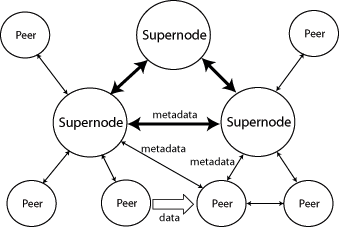
\includegraphics[width=0.5\textwidth]{src/img/p2p-systems/fasttrack}
  \caption{FastTrack Architecture}
  \label{fig:p2p-systems:fasttrack}
\end{figure}

The number of nodes defined as Super-Nodes may vary from tens to hundreds.
This happens because Super-Nodes are ordinary nodes that can enter or leave the
network when they want. As a result, the network is dynamic and in constantly
changing. To ensure constant availability, the presence of several nodes is
required. Such nodes are called bootstrap nodes and must always be active
(online). When a FastTrack client (for example Kazaa) is running on a node, it
will initially contact the starting node. Next, the starting node will
determine if that node can be considered a Super-Node. If so, it will be given
some (or perhaps all) of the IP addresses of other Super-Nodes. If it
classifies as a common node, then the starting node will respond by providing
the IP address of one Super-Node.

Some clients (like Kazaa) use a method named reputation system. Reputation is
associated for each user and is reflected by the level of participation (a value
between 0 and 1000) in the network. The longer a user is connected, the higher
the level of participation is, such that it will be favored in priority
policies and will receive the best services. This measure aims to encourage
users to share files and reduce the number of ``passengers clients'' on the
network.

Resources are discovered through diffusion between Super-Nodes. When a node
from the second level makes a request, it is directed through the partner
Super-Node that will send the request to other Super-Nodes connected with it.
Diffusion is repeated until TTL's value reaches 0. This provides the FastTrack
client with a greater coverage and best search results. A disadvantage is the
resource usage of the method of diffusion that may lead to a significant load
of bandwidth between Super-Nodes. However, this problem is not as serious as
is the case for Gnutella and Kazaa due to fast available connections of
Super-Nodes.

Each request received by a Super-Node is searched through the database. The
database contains information about all files shared through the network. When
a match is found, a reply is send on the same path to the original node. The
method is similar to response propagation in Gnutella network. However, the
problem of packet loss is not as severe as in Gnutella. In Gnutella, the
backbone consists of nodes that connect and disconnect from the network at
will. In FastTrack, the backbone consists of nodes with high connectivity
speed (Super-Nodes) and, therefore, return paths may be considered safer.

\subsection{eDonkey Network}

The eDonkey network is a centralized P2P file sharing system. Several central
servers maintain information about various shared files, following the actual
transfer of files that take place directly between nodes.

eD2K original protocol was not formally documented. However, given that most
of today clients (\textit{*Mule}) are open-source, it can be said that the
formal specification for eDonkey network is defined by how eMule client and
eDonkey server interact. By running an eDonkey server on a system with
Internet connection, any user can add a server in its network. Clients
frequently update their local list of servers as IP addresses continue to
change.

eDonkey network files are uniquely identified by a MD4 summary. This means
that files with identical content but different names are the same. Files are
divided into "blocks" of 9,728,000 (9500 x 1024) bytes plus a residual block.
For each block a MD4 checksum of 128 bits is computed. This way an error is
detected in transmission and corruption is achieved only at block level, not
at the file level. In addition, successfully downloaded blocks are available
for file sharing before the entire file is downloaded (similar to the
BitTorrent protocol).

Initially, the eDonkey protocol used a set of servers provided by users who
donated the necessary bandwidth, processing overhead and disk space. Such
servers generates heavy traffic and, as a consequence, were more vulnerable to
attacks.

As a result, Overnet was developed by MetaMachine, the initial developer of
eDonkey client, and Kademlia was developed by eMule project.

Kademlia is the version without server from eDonkey network, similar to
Gnutella.  Unlike Gnutella, Kademlia uses distributed hash tables (DHT -
Distributed Hash Tables) to store information about files across the network.
Thus, while Gnutella search operations were achieved through ``flooding'' the
network with \textit{Query} messages, Kademlia searching is performed on a
hash function that allows identify nodes where information about location of
the files is recorded. Locality information is stored in several nodes to
allow entering or leaving the system without losing location information.

Joining the network is achieved, as in the case of Gnutella, through a bootstrap
node, known from the beginning by Kademlia client.

\subsection{DirectConnect}

DirectConnect is a centralized protocol for P2P file sharing. Its architecture
is similar to Napster, but while Napster was using a single central server
(and therefore a unique point of failure), DirectConnect provides multiple
dedicated servers called hubs where clients can connect.

DirectConnect is a text protocol, commands and information being sent in clear
without being encrypted. As clients connects to a central source of
distribution of information, the hub must have substantial bandwidth.

There is no official specification for the protocol. This means that each
client or hub obtained information about functionality by breaking the
original protocol (reverse engineering).

The P2P part of protocol is based, as in eDonkey's case, on the concept of
slot, a number that denotes the number of users that can simultaneously
download files from the current user. These slots are controlled by the
client. Downloads use TCP while active requests use UDP. A client may find
itself in on of two states: active or passive. Clients in the active state may
download from anyone else in the network. Clients in the passive state may
only download from active users.

Hubs hold information about clients and possess features such as searching and
chat. File transfer takes place directly between clients, as in a common P2P
system. Many hubs impose requirements related to the number of files its
members can share and restrictions on the quality and the content of shared
files. Additionally, a hub may choose some users as operators to maintain
certain rules. One problem of DirectConnect hubs is scalability,
central-server architecture preventing this.

\subsection{Instant Messaging. Jabber/XMPP}

One of the most common forms of P2P applications is instant messaging. During
the early age of the Internet, e-mail was inherently Peer-to-Peer. The message
was sent by making a connection from a user terminal to another terminal.
However, over time, communication between users became an indirect one. Most
personal computers could not support communication protocol and used dedicated
servers (MTAs -- \textit{Mail Transfer Agents}) for sending messages.

One problem of e-mail service was that it didn't act as a real time service.
Messages could be delayed or even lost. The result was the appearance of
chat applications that allowed real-time communication. At the beginning,
applications emerged in which communication was mediated by servers
(server-relayed chat). An example is IRC (Internet Relay Chat). This type of
application is not Peer-to-Peer. However, IRC is the precursor of P2P user type
that allowed nodes to discover and initiate contact using other client
technologies.

The term ``chat'' is, by confusion, used for broadcasting transmission for
multiple users (broadcast relay) and for private messages transmitted over a
point to point connection. A separate group of applications are dedicated to
the second category. In other words, ``instant messaging'' refers to different
types of chat that imply connectivity between communicating nodes.

The main purpose of Jabber/XMPP (eXtensible Messaging and Presence Protocol)
is a ``technology of conversation'' for P2P in the general sense, including
not only user-user communications, but also user-application or
application-application. Jabber evolved as a project that brings about various
applications to create an open and distributed P2P architecture as a basis for
specialized actions. The design involved choosing XML as a consistent way of
encapsulating information, regardless of application, and allowing the
addition of extensions. Applications are implemented in XML and translated
transparently in the native format.

Some other projects developed in Jabber are:
\begin{itemize}
  \item gateway for most instant messaging protocols;
  \item libraries most of programming languages;
  \item a modular open-source server and clients for any platform;
  \item a number of specialized server functions such as language translations.
\end{itemize}

A special emphasis is given to user-applications and to designing a protocol
that facilitates all forms of P2P communication. First application of Jabber
technology is an instant messaging system that takes into account security,
usability, network accessibility (from anywhere, using any type of device) and
interoperability with Web services of instant messaging or telephone.

In the center of the open architecture lies the idea that communication takes
place using XML format, enabling Jabber to work both as a storage service and
as a replacement. Meta-information and structure are similarly defined in XML
and possess established sets of tags to describe document files, audio, video,
etc. Although Jabber can be used with multiple purposes, the most common
implementation is an instant messaging client.

\subsubsection{Infrastructure}

The inspiration model for Jabber is e-mail: a distributed network of servers
that use a common protocol and connect several clients in order to allow
message exchange (sending and receiving). The main functional difference
between Jabber and e-mail is real-time communication and the incorporation of
presence information, unlike the ``store and send'' approach from e-mail
service.

Servers are totally independent of each other and maintain their own list of
users and services. Messages are transferred to a P2P atomistic network. Any
number of Jabber servers may form a network. A particular user is associated
with a specific server and an identity that appears as an e-mail address
(such as \texttt{george@jabber.org}). This identity is created either when
initiating the registration process or during an administrative configuration
of the server.

A Jabber application can expose internal data to the general public. An
external URI could have a format such as
\texttt{jabber://user@server/resource/data}.

\subsubsection{Jabber Clients and Servers}

On one hand, Jabber is primarily a client-server architecture. Clients
connects to a Jabber server before any P2P transfer. Also, Jabber chat
messages are routed through the server. Each session creates a ``stream of XML
communication'' to the contacted server, a flow that takes the form of an
online session.

Direct connections between nodes are defined as application specific: they are
perfectly possible, but must first be negotiated in the context of
a client-server paradigm. A part of Jabber's design decision was to move the
complexity to a server component. Developers may then create new clients very
easily and system administrators can easily add new functionalities without
massive upgrades of client applications. Jabber server core is relatively
small such that each system may have its own Jabber integrated server, that,
from a user point of view, would be equivalent to an atomistic P2P system.

Using XML is an important part of architecture as XML tags can express any
structured information. All Jabber components must be able to communicate using
XML, even when the information transferred could use other protocols.

\subsubsection{The Jabber Protocol}

Jabber specific messages form three types of XML messages: message, presence
and info/query (\texttt{iq}). The structure and syntax are very simple and the
format is text. An example is:

\begin{verbatim}
<message to='user@server' type='chat'>
    <body>The actual text of the message.</body>
</message>
\end{verbatim}

A \texttt{from} field is added by the server when the messages are
transmitted. The type is optional and reduce to a common message. Type
\texttt{chat} means that the client displays this message in a chat windows.
Other message elements are: \texttt{html}, \texttt{subject}, \texttt{thread}
(to keep information on replies), \texttt{x} (used for extensions).

\subsection{P2P Collaborative Spaces. JXTA}

Many of innovative aspects of the Internet have evolved as a result of the
desire of people to collaborate regardless of their location.  Peer
technologies are natural solutions for informal collaboration and encourage
the formation of collaborative groups of people. In the absence of physical
presence, many people need working together and it is vital that there are no
barriers in the way of effective communication. P2P informal groups are among
the best suited mechanisms of work.

Moreover, these informal groups are widely used by many people, regardless of
formal structures that can be centrally imposed. The trend is so intense that
people don't realize what is happening. When will be asked, they will say that
they work as in a working methodology from a hierarchical structure. However,
studies performed by external group persons shows a rapid succession of
contacts in P2P format.

JXTA project (short for \textit{juxtaposition}), or side by side, is a Sun
Microsystems initiative that seeks to integrate P2P technology as
complementary tools distributed in Internet. The basic platform is a fully
decentralized network architecture. However, both centralized and
decentralized services can be developed over the platform.

\subsubsection{JXTA Architecture}

On JXTA architecture, arbitrary network entities try to discover other network
entities and to collaborate with them. There is no need for any media support
of any of the participants but it has to present the form and the content of
discovery exchanged messages in the network.

The architecture is described using three levels:

\begin{itemize}
  \item \textbf{application level}: supports implementation of integrated
  applications such as file sharing, resource sharing and storage;
  \item \textbf{service level}: providing API interception for generic network
  services, commonly used in P2P applications; examples include searching,
  sharing, security features;
  \item main level (core layer): implements protocols and essential components
  for P2P networks; this level includes node discovery, a transport level with
  specifications that include firewalls and security issues.
\end{itemize}

The entire design is modular and allows developers to choose services or
applications that match their needs. The common core allows services to be
interoperable and applications developed to mix and match the desired
characteristics using existing or new modules.

\subsubsection{Groups and Nodes}

In the context of JXTA, nodes are defined as devices that know at least one
part of project JXTA protocols. The definition may include a large number of
devices such as servers, PCs, PDAs, mobile phones and embedded devices. The
only requirement is that nodes must be connected to a network type (IP,
Bluetooth, etc.).

A group is a collection of nodes with a common set of rules for
intercommunication. Each group can set its own policies for members: from
fully opened to very safe and protected groups.

In JXTA terminology, Java objects used in transmission, containing code and
data, are called coded objects.

\subsubsection{Security Model}

The security core of the JXTA project is implemented using encryption schemes
and public keys / private keys signatures. Such a system provides strong
security provided it is implemented in a "trusted" context.

The trusting model, called "P2P Web of Trust", is similar to the name "Web of
Trust" used by PGP to secure e-mail and is used for transferring public keys
between members. Each member is mapped a certain level of trust, formal or
informal. Keys signed by trusted members gain their own trusted status. A
policy group may grant authority to certain members to sign other members'
public keys, in addition to routine tasks such as authentication and adding or
removing members.

There are security classes for usual algorithms (RSA, RC5, SHA-1). Combinations
of classes form groups of security implementations.

\subsubsection{Projects Using JXTA}

The main components of JXTA are developed in a different separate projects:
jxme (mobile platforms), jxta-c, jxtaperl, jxtaruby, platform (for Java SE),
pocketjxta, security.

JXTA core services include authentication, discovery and coded management.
Other services include the name, routing, coded searching and indexing.

CMS: JXTA implements a Content Management Service with sharing across a group.
InstantP2P applications use CMS to implement searching, sharing and shell
commands sharing.

Edutella project uses a P2P network to exchange educational resources between
various universities. The vision is to provide meta-information services,
necessary to enable interoperability between heterogeneous JXTA applications.

JxtaVFS project aims to manage virtual files, representing dynamic files mapped
over remote resources; is a way of creating a distributed and hierarchical map,
self-sustained by resources within the network.

Payment Project aims to implement EPocketCash protocol for financial
transaction which permit users to become buyers or sellers on the same account.

JXTA applications allow interactive acces to P2P JXTA platform. Many of then
use little storage space. JXTA Shell is an optional command line interpretor
that allows users and developers to interact with JXTA platform. Gnougat is a
Gnutella service implemented over JXTA technology.

There are a big number of projects in development. JXTA should be viewed as an
alternative platform, decentralized, with open-source P2P functionality that
can reach or exceed the centralized vision of the closed .NET platform.

\section{BitTorrent}
\label{sec:p2p-systems:bittorrent}

One of the disadvantages of P2P systems is the ``opening'' for \textit{free
riding}~\cite{free-riding} or \textit{free loading}. While peers are generally
considered to be altruistic, this behavior is not generally enforced. Free
riding is equivalent to an egoistic behavior, where a peer gets information
from other peers and gives nothing back. This behavior disables the very
nature of P2P systems: sharing information.

If a given network consists of a high number of free riders, then data load
among peer is unbalanced. When a new node shares a popular file in the native
P2P system, it will attract a large number of connections. In case of free
riding, this node must provide bandwidth for additional clients.

BitTorrent is a new protocol being used to solve the free riding problem,
though not completely~\cite{free-riding}. The idea behind the protocol is
fairly simple: the node that plays the role of the server breaks the file in
pieces. If the file is requested by more clients simultaneously, each client
will get a different piece of that file. When a client gets a complete piece
it will allow other clients to download that subfile, while it will continue
downloading the second piece. In other words, the node acts simultaneously as
a client and a server after receiving the first piece. The process continues
until the download completes.

The BitTorrent protocol is highly suitable for downloading large files where
the download process takes a long time. As a direct consequence, more
``server'' peers are available for a longer duration. More clients will not
result in a performance decrease of the whole network as the load is
distributed.

Figure~\ref{fig:p2p-systems:bittorrent-sharing} show a diagram of a sharing
process among several peers. The ``server'' possesses 4 pieces. Each clients
on piece from a server at a given time. As noticed, client \#1 gets all pieces
but from different nodes. The order pieces reach the client may not respect
the initial piece succession. The BitTorrent algorithm will try maximizing the
number of pieces available for download at a certain point in time -- that is
balancing the availability of pieces among peers in a network.

\begin{figure}
  \centering
  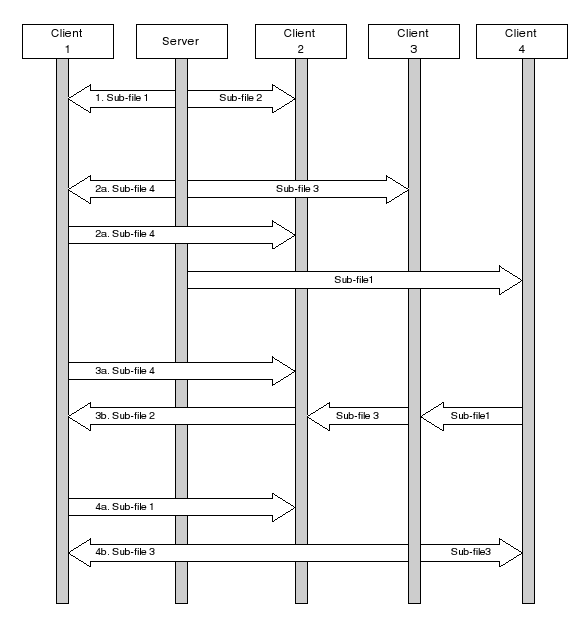
\includegraphics[width=0.4\textwidth]{src/img/p2p-systems/bittorrent-sharing}
  \caption{BitTorrent File Sharing}
  \label{fig:p2p-systems:bittorrent-sharing}
\end{figure}

In order to download a file in BitTorrent network, the user would follow the
step below:

\begin{itemize}
  \item install a BitTorrent application;
  \item surf the web;
  \item find a file on the server;
  \item select location where the file would be saved;
  \item wait for completion of the process;
  \item instruct application to close (the upload process, also called
  ``seeding'' continues until the user closes the application).
\end{itemize}

\subsection{BitTorrent Keywords}

A \textit{peer} is the basic unit of action in any P2P system, and, as such, a
BitTorrent system. It is typically a computer system or program that is
actively participating in sharing a given file in a P2P network. A peer is
generally characterized by its implementation, download/upload bandwidth
capacity (or limitation), download/upload speed, number of download/upload
slots, geolocation and general behavior (aggressiveness, entry--exit time
interval, churn rate).

The context in which a BitTorrent content distribution session takes place is
defined by a BitTorrent \textbf{swarm} which is the peer ensemble that
participate in sharing a given file. It is characterized by the number of
peers, number of seeders, file size, peers' upload/download speed. A healthy
swarm, one that allows rapid content distribution to peers, is generally
defined by a good proportion of seeders and stable peers (peers that are part
of the swarm for prolonged periods of time).

A swarm consists of two types of peers: leechers and seeders. A
\textbf{seeder} is a peer that has complete access to the distributed content
and is, thus, only uploading data. A \textbf{leecher} has incomplete access to
distributed content and is both uploading and downloading. The BitTorrent
negotiation protocol uses a form of tit-for-tat that forces peers to upload in
order to download (though this has been proven to be
abused~\cite{free-riding}) therefore ensuring fairness and rapid distribution.
A good number of healthy seeders is a requirement for healthy swarms that
allow rapid distribution of data.

A swarm is given birth by an \textit{initial seeder} which is the peer sharing
a file it has complete access to. The seeding/sharing process within a swarm
is started through a metafile, a \textbf{.torrent} file, that defines swarm
trackers and piece hashes to ensure content integrity. Typically, a peer uses
a web server to download a .torrent file and then uses a BitTorrent client to
interpret it and take part into a swarm. It is possible to create different
swarms for the same content by using different trackers in a .torrent file.

Communication of peers in a swarm is typically mediated by a BitTorrent
\textbf{tracker} or several trackers which are defined in the .torrent file.
It is periodically contacted by the peers to provide information regarding
piece distribution within the swarm. A peer would receive a list of peers from
the tracker and then connect to these peers in a decentralized manner. As it
uses a centralized tracker, the swarm may suffer if the tracker is
inaccessible or crashes. Several solutions have been devised, such as PEX
(Peer EXchange)\footnote{http://wiki.vuze.com/w/Peer\_Exchange} or DHT (Distributed Hash Table)~\cite{dht-paper}.

\begin{figure}[htb]
  \begin{center}
    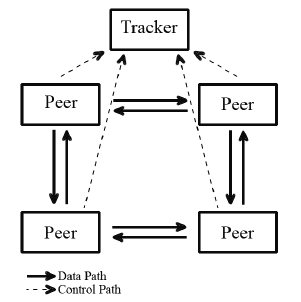
\includegraphics[width=0.4\textwidth]{src/img/p2p-systems/bittorrent-overview}
  \end{center}
  \caption{Overview of BitTorrent Components}
  \label{fig:p2p-systems:bittorrent-overview}
\end{figure}

As shown in Figure~\ref{fig:p2p-systems:bittorrent-overview}, there are two
types of communication paths. The control path is established between each
client and the tracker to request information about other peers in a swarm.
The data paths are typical paths used between peers. Peers exchange
information according to the internal BitTorrent algorithm.

\subsection{BitTorrent Internals}

The core of the BitTorrent protocol is the \textit{tit for tat} mechanism,
also called \textit{optimistic unchoking} allowing for upload bandwidth to be
exchanged for download bandwidth. A peer is hoping another peer will provide
data, but in case this peer doesn't upload, it will be \textit{choked}.
Another important mechanism for BitTorrent is \textit{rarest piece first}
allowing rapid distribution of content across peers. If a piece of the content
is owned by a small group of peers it will be rapidly requested in order to
increase its availability and, thus, the overall swarm speed and performance.

The usage of the rarest piece first algorithm means that pieces in a file
would be equally distributed among peers in a swarm and provide rapid access
of each of those. This approach has the down side of not providing data
sequentially which is troubling for streaming applications. In such
applications the algorithm is updated to use priority sets and only pieces
that are not prioritized to be fetch in a ``rarest piece first manner''.

In order to allow client bootstrapping and access to pieces information,
initial peers must be able to gather some initial data without giving anything
back. In order to accomplish this bootstrapping phase, BitTorrent provides an
``optimistic unchoke'' slot to each client. This is also useful for
establishing potentially better connections than the ones currently used.

The use of choking and unchoking is the tit-for-tat variant of the BitTorrent
protocol. Peer reciprocate uploading to peers which upload to them, with the
goal of having multiple connections actively transferring in both directions.
Clients choose peers to choke or unchoke based on their current transfer rate,
such that connections used would tend to be the best available from a download
speed point of view.

\section{Content Distribution in Peer-to-Peer Systems}
\label{sec:p2p-systems:streaming}

Peer-to-Peer solutions have traditionally been used for file sharing among
users in the Internet. Generally, file transfer occurs in small chunks (also
called pieces) that are transferred or exchanged from one client to the other.
Two different pieces may be transferred from two different clients, depending
on their availability. Piece transfer may not be (and generally isn't)
sequential; that is, a piece is transferred according to its availability,
peer approval and implementation of the Peer-to-Peer protocol.

As multimedia content forms a large part of data that is distributed over the
Internet, recent years have witnessed the rise of streaming solutions and
their introduction to Peer-to-Peer solutions. Both live streaming and
on-demand video streaming have been added to existing Peer-to-Peer solutions
of new applications have been designed. We introduce the main methods for
providing streaming solutions for P2P systems, such as tree, multi tree and
mesh based systems.

Streaming video over the Internet has mostly relied on a client-server
paradigm. A client connects to a stream server and video content is streamed
from the server directly to the client. A specialized variant of the
client-server model is the Content Delivery Network (CDN). In CDN-based
solutions, the video source server pushes the content to a set of delivery
servers which are subsequently accessed by clients. Such technology is
employed by YouTube.

\subsection{Peer-to-Peer Streaming}
\label{subsec:p2p-systems:p2p-streaming-p2p}

In a P2P network the user may not only download a video asset, but he/she may
also upload it. Thus a user becomes an active participant in the streaming
process. Recent years have seen the emergence of video streaming applications
based on P2P solutions.

P2P streaming solutions~\cite{p2p-streaming-survey} create an overlay network
topology for delivering content (that is, a virtual network topology over a
physical one).  The overlay network typically follows one the two structures:
\textit{tree-based} and \textit{mesh-based}.

In a tree-based topology data is pushed from its \textit{root node} to
children nodes, then to other children nodes and so on. Its main disadvantage
relies with peer departure (peer churn). A peer departure will temporarily
disrupt video delivery to child peers of the departed node.

A mesh-based topology, peers are able to communicate with other peers without
having to adhere to static topologies. Peer relations are established based on
data availability and network bandwidth. A peer periodically initiates
connections to other peers in the network and exchange information regarding
data availability and pull data from neighboring peers. It allows the
advantage of robustness to churning. It does, however, suffer from video
playback quality degradation with no clear data distribution path.

As will be described below, mesh-based systems and tree-based systems are used
both for live streaming and video-on-demand depending on protocol internals
and application design.

\subsection{Video-on-Demand}
\label{subsec:p2p-systems:vod}

Video-on-Demand (VoD) ensures the availability of the whole video at the time
of the transfer. No content is generated/updated while data is transferred and
rendered. It allows users to watch any point of video on any time.

As peers in a given network are playing a different part of the file, pieces
of that file have to left available for other potential peers. One peer may
discard pieces of the VoD asset as time goes by or preserve the whole file for
seeding. While mesh-based topologies are usually enabled for VoD delivery,
tree-based topologies still find their way.

A tree-based P2P VoD service groups users in sessions based on their arrival
time, using a threshold. Users that arrive close to that time (within the
threshold) constitute a session. The server streams the video over the base
tree as in tree-based P2P live streaming. Users cache certain pieces/patches
of the video to make it available to other users. Users will thus provide two
functionalities: \textit{base stream forwarding} and \textit{patch serving}.

\begin{figure}
  \centering
  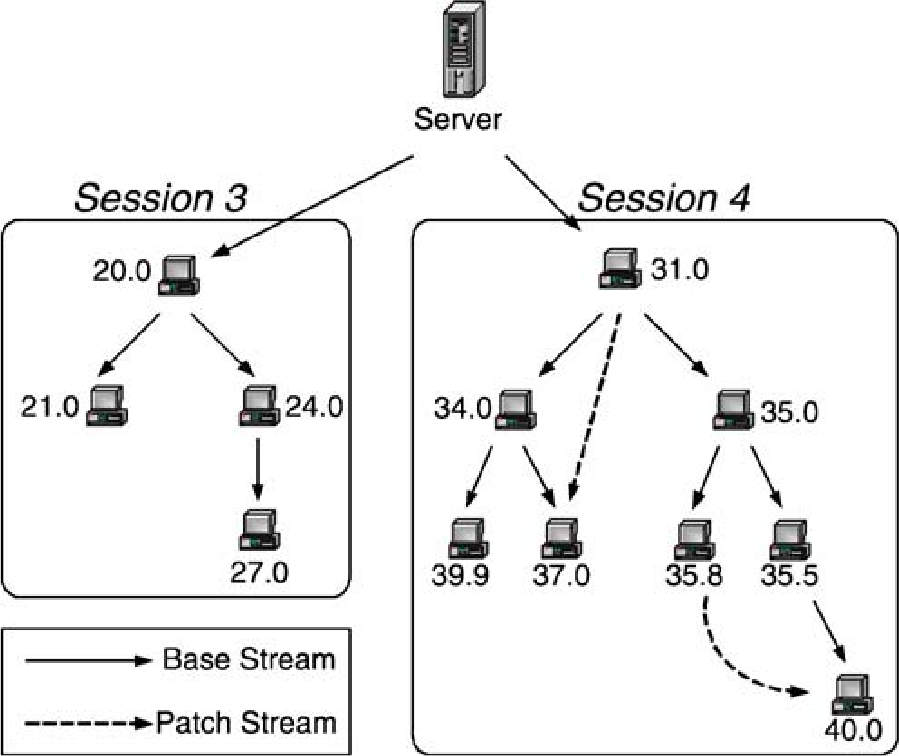
\includegraphics[width=0.5\textwidth]{src/img/p2p-systems/tree-based-vod}
  \caption{Tree-based Video-on-Demand}
  \label{fig:p2p-systems:tree-based-vod}
\end{figure}

In Figure~\ref{fig:p2p-systems:tree-based-vod}, there are two sessions (3 and 4) starting
at time 20.00 and
31.0, respectively, with a threshold of 10. Each user is maker with its
arrival time in the system. A straight arrow is used to represent a base
stream while a dotted arrow is a patch stream. Each user may receive
information from multiple users and it could also send information to multiple
users.

Mesh-based P2P file sharing network uses swarming (a collection of peers) and
is suitable for BitTorrent protocols. In a mesh-based network, peers connect
to other available peers depending on various factors such as availability,
bandwidth and protocol internals. Data delivery is highly similar to a
BitTorrent environment: there are seeders that possess all data and leechers
that possess only a subset of information. Data is fragmented into pieces and
is subsequently deliver (upon request) to various peers.

One of the first attempt to design a mesh-based P2P VoD service what
BiToS~\cite{bitos}. There are three components within the piece processing
activity in BiToS, as seen in Figure~\ref{fig:p2p-systems:bitos-vod}: the
receive buffer, consisting of all received information so far, the high
priority set, consisting of pieces that are required to allow smooth
prerendering and the remaining set. The optimal allocation of resources is an
important design challenge.

\begin{figure}
  \centering
  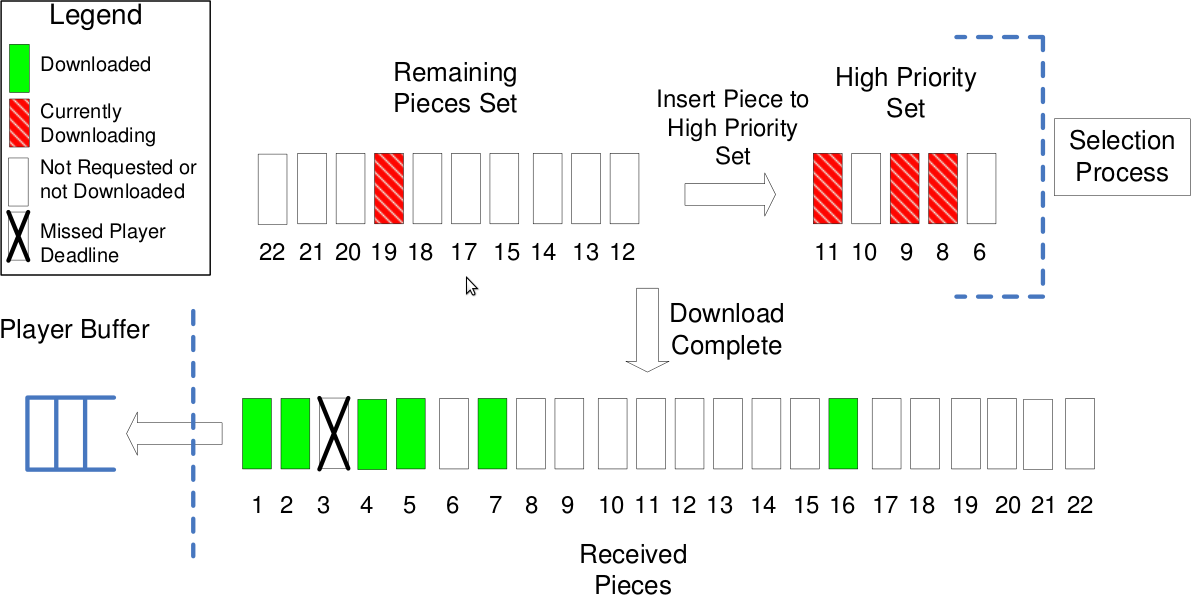
\includegraphics[width=0.7\textwidth]{src/img/p2p-systems/bitos-vod}
  \caption{Video-on-Demand in BiToS}
  \label{fig:p2p-systems:bitos-vod}
\end{figure}

\subsection{Live Streaming}
\label{subsec:p2p-systems:ls}

Live streaming consists of a server that is generating video content in real
time. Content dissemination is acted upon by other peers (clients). The video
playback is synchronized among all peers unlike peers in a VoD-like network,
where each peer may be positioned in a different part of the video.

Live streaming is usually making use of tree-based structures. A root server
is constantly (real-time) generating content and peers connect as clients
forming a tree. One of the basic frameworks for creating a tree-based overlay
is the deployment of IP level multicast. Due to implementation lack of
adoption, the IP level multicast hasn't been deployed and the multicast
function has been implemented at application level. A tree-based approach
could either be using a single tree streaming or multi-tree streaming.

In a single-tree streaming
(Figure~\ref{fig:p2p-systems:single-tree-streaming}), a tree is formed at
application level based on the root node which is equal to the server. Each
user is a client and, subsequently, a server and is joining the tree at a
certain level. It receives the live stream from the above node and delivers
the information to the children peers. A node receives data from a single
parent node but may deliver it to multiple nodes.

\begin{figure}
  \centering
  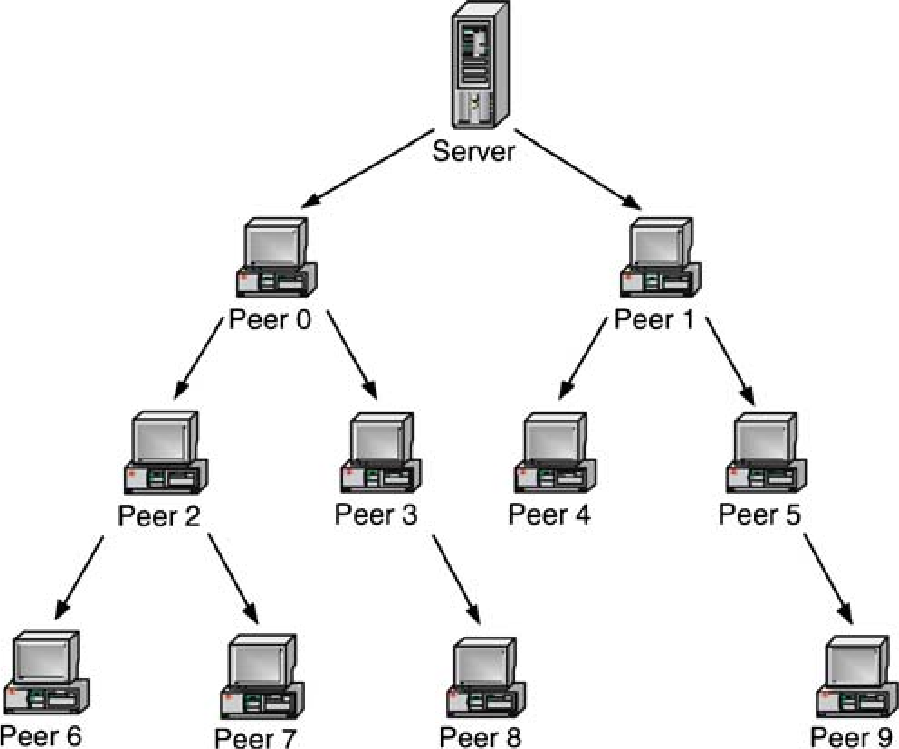
\includegraphics[width=0.5\textwidth]{src/img/p2p-systems/single-tree-streaming}
  \caption{Single-tree Streaming}
  \label{fig:p2p-systems:single-tree-streaming}
\end{figure}

An important issue of single-tree streaming is its construction. One would
required a small fan out and a small number of tree levels. A small fan out
would imply that nodes use their upload bandwidth to provide information to a
small number of nodes. A small number of levels means reduced delay in
propagating the streaming. As one can not achieve both a small number of
levels and a small fan out, compromise must be taken into account. Typically,
one would decide on the upload bandwidth available, compute the maximum fan
out and construct the tree accordingly. As more nodes are part of the network,
the number of levels would increase.

Another important issue is tree maintenance. Churning is an integral part of
a Peer-to-Peer network. Peers are dynamic and may leave the network (either
gracefully or unexpectedly). The child peers are not able to stream and the
tree has to be reconstructed as fast as possible. This is possible by
reassigning the peers to the server (similar to the arrival of a new peer).
The recovery may be done through the decision of a centralized server or in a
decentralized fashion.

The single-tree approach does possess important drawbacks. One of them is that
such a topology can not recover fast enough for frequent peer churn. Another
drawback is the lack of contribution from leaves. Leave peers don't put up use
of their upload bandwidth as no other peers are connected to them and request
streaming information.

The issue of leaf nodes is addressed through the use of multi-tree based
approaches. A server divides the streamed information in sub-streams. Each
peer joins all substreams, and information is flowed from the root node to
leaf nodes. A node may not (and usually is not satisfactory) be places in the
same position in each of the trees. In a given tree the node may be a leaf
node, meaning that it would only receive information from a substream; in
another substream it could be placed as an internal node. In the latter
substream the node would thus be able to use its upload bandwidth to provide
information to other peers. Multi-tree based systems would still suffer from
peer churning and tree maintenance has to be taken into account.

\subsection{Existing Solutions}
\label{subsec:p2p-systems:solutions}

Several commercial solutions have been developed around the concepts of
Peer-to-Peer streaming, making use of the scalability benefits and low cost
for distribution.

One of the most successful media streaming platforms,
Octoshape\footnote{http://www.octoshape.com/} uses various optimizations to
deliver high quality streaming to users.  Octoshape was responsible for
allowing the streaming of the US Inauguration of President Barack Obama or the
wedding of Prince William to Kate Middleton.  Octoshape uses a strategic
partnership with different CDNs allowing a distribution grid that minimizes
cost but also ensure HD content availability to average users. Its similar to
a Peer-to-Peer engine that uses a plethora of high quality peers to deliver
content all over the world. Its optimizations range from using a specialized
Octoshape streaming protocol, multiple point failover, loss resilience, a
secure suite of multicast technologies.

While not a Peer-to-Peer streaming application,
Akamai\footnote{http://www.akamai.com/} is an extended content delivery
network that positions servers in various locations to allow rapid access.
Akamai created a globally distributed network of tens of thousands of servers
which is controlled by proprietary software.  Akamai servers typically mirror
content which is subsequently server to users.  Akamai clients provide their
content to Akamai servers which mirror and distribute it across the Akamai
network. Users would typically access the server which is closest to their
location.

Peer-to-Peer video streaming networks are PPTV and PPS.tv. Both are Chinese
oriented solutions. PPS.tv uses 8.9\% of the market share in China. Through
the use of P2P-streaming it supports high-volume traffic, allowing several
hundred users to watch a live stream at 300-500 Kbps with a server possessing
only 5-10 Mbps. PPTV offers both live streaming and video-on-demand, covering
a large specter of video assets for Chinese audience. Recently, the PPLive
team behind PPTV has migrated to a hybrid CDN-P2P cloud technology, called
PPCloud, considered as scalable and cost-effective. Several other solutions
have failed to gain momentum due to legal issues and locality constraints.

BitLet\footnote{http://www.bitlet.org/}, an abbreviation for BitTorrent Applet
is a BitTorrent program enabling the use of the file sharing protocol inside a
Java-enabled web browser. The client download and uploads content as long as
the program window is open. As a specialized functionality, BitLet allows
streaming audio; it also possesses an experimental streaming video feature
(based on Theora).

RTMFP\footnote{http://www.adobe.com/products/flashmediaserver/rtmfp_faq/} is a
proprietary protocol developed by Adobe Systems that enables direct
Peer-to-Peer communication between multiple Adobe Flash Players and
applications build using Adobe AIR framework. RTMFP retains the benefits of
P2P-based streaming such as reduced bandwidth cost and scalability.
Cirrus\footnote{http://labs.adobe.com/wiki/index.php/Cirrus} is the technology
that enables peer assisted networking using RTMFP within the Adobe Flash
platform. Cirrus 2, available in Flash Player 10.1, supports groups, allowing
application-level multicast and reducing the load on the source publisher.

BitTorrent DNA\footnote{http://www2.bittorrent.com/dna} (\textit{BitTorrent
Delivery Network Accelerator}) is a program designed to speed up viewing of
streaming video through the use of the BitTorrent protocol. BitTorrent DNA is
UDP based, replacing regular TCP-based bandwidth throttling with a much more
sensitive technique. Users will be able to download pieces of content from
other users, releasing bandwidth pressure from the original content source. It
is targeted at streaming and online video games.

\section{Issues and Challenges in Peer-to-Peer Systems}
\label{sec:p2p-systems:issues}

The plethora of Peer-to-Peer solutions in the Internet makes it difficult to
choose the best one for a given job. Each application or application type is
specialized in a given kind of activity; variations of each kind of
application is itself an issue when aiming to use the best one. Measurements,
metrics and evaluations have to be considered to allow a formal classification
of these solutions.

Streaming (both VoD and live) has been integrated into many Peer-to-Peer
solutions.  However, performance has been reported to still lag behind a
medium-load HTTP streaming server and far behind a classical \textit{Content
Delivery Network} (CDN). Better bandwidth utilization, increased peer
incentive, new business models and hybrid P2P/CDN infrastructures may provide
increased performance for Peer-to-Peer applications when dealing with
streaming requests.

In order to provide an evaluation of various Peer-to-Peer solutions out there,
one would either turn to experimentation and validation or through formal
analysis. While formal analysis is achievable through a ``pen and paper''
approach, experimentation requires a high number of resources and carefully
placed ``information probes'' to gather information. A common approach
involves ``hooking'' probes in existing Peer-to-Peer swarms and gather
information in those points. Another one involves creating an infrastructure
that is able to realistically simulate a Peer-to-Peer network; this approach
would, however, require a large number of systems, close to the size of an
average swarm -- in order to ensure a realistic trial environment.

Apart from the technical challenges surrounding a Peer-to-Peer based solution,
issues are constantly in place regarding legal aspects of data distribution.
As most of the content is owned by publishing houses, even tens of years after
its creation, it's implied transferring much of that content is illegal. A
typical BitTorrent network doesn't integrated features such as encryption, DRM
and ownership information, meaning that it is highly plausible that, by acting
to download a piece of content, you come across a legal aspect. Often vague
and inconsistent legislation only adds to the problem. The plethora of legal
issues concerning BitTorrent is made apparent by the high number of legal
disputes regarding various distribution sites, one of the most famous being
``The Pirate Bay''\footnote{http://thepiratebay.org/}. Various Peer-to-Peer
streaming solutions have failed to gain momentum or have even been
closed/disabled due to legal troubles.

The legal aspects of Peer-to-Peer streaming solutions incur a greater
difficulty in providing a successful business model. There are two approaches.

A first approach is one that considers using a proprietary and secure platform
that selectively transfers information to users, possibly in an encrypted
form, such that other users in the swarm may not access that information. This
approach would be adequate to large media creators that want to deliver their
content to users but want to keep information private and only paying users
would access that -- as it is typical in CDN-based solutions such as Akamai.

The second solution takes into account that protecting content ownership and
making profit out of it is not a priority. Rather making profit from side
activities such as commercials, user credits, premium content, social
networking solutions. This model is close to the functionality provided by
YouTube where all content is available, a user may choose to ingest content
and profit is taken out of commercials. The selective insertion of commercials
into video streams is a possible solution for making profit out of ``free''
content into Peer-to-Peer networks.

There are still lingering questions regarding the possibility of success for
any of the above solutions. Given the vague legislation and continuous debates
between anti and pro-piracy groups, a suitable solution is yet to come out.

Even after 10 years of continuous development, Peer-to-Peer systems raise
interesting questions and pose significant challenges to Internet scientists
and engineers. Thorough analysis and evaluation coupled with cleverly
designed and efficient solutions are key to improving Peer-to-Peer
applications and their usage in the Internet.
